\documentclass{article} % For LaTeX2e
\usepackage{nips15submit_e,times}
\usepackage{hyperref}
\usepackage{url}
\usepackage{graphicx}
%\documentstyle[nips14submit_09,times,art10]{article} % For LaTeX 2.09


\title{Weekly Report(March.4,2019-March.10,2019)}

\newcommand{\fix}{\marginpar{FIX}}
\newcommand{\new}{\marginpar{NEW}}

%\nipsfinalcopy % Uncomment for camera-ready version

\begin{document}

\maketitle

\begin{abstract}
This week I learned a lot about FullyNeuralNetwork, Batch Normalization and Dropout. 
I understand more about neural network through this week's learning.
\end{abstract}

\section{Learned}
I learned more about NN, and I get a clearer understanding about it.

\subsection{FullyConnected Neural Network}
There are more than two layers, but each two contiguous layers are all connected like the two-layers neural network implemented in assignment1. In the hidden layer, as usual we use ReLu as activation function. Output Y is activated by softmax function. By this way, we can also assume it as probability.

Form ( L layers):
\begin{center}
{affine - [batch/layer norm] - ReLu - [dropout]} * (L - 1) - affine - softmax
\end{center}

\begin{figure}[h]
	\centering  %插入的图片居中表示
	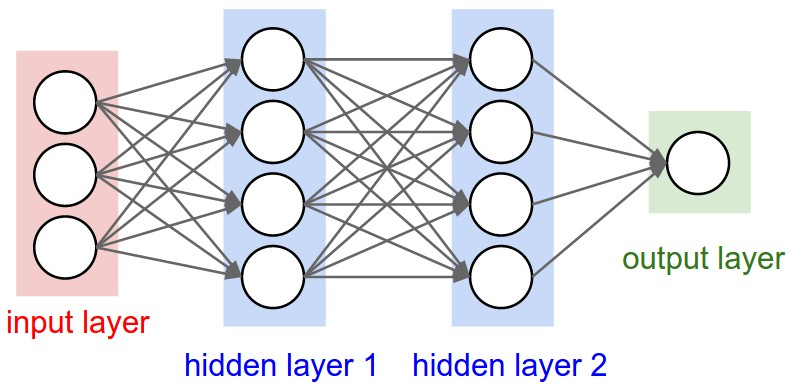
\includegraphics[width=.4\textwidth]{3.jpg} 
	\caption{2-dimension}  %图片的名称
	\label{fig:f3}   %标签,用作引用
\end{figure}

\subsection{Batch Normalization}
Advantages:

1.avoid saturation of activation function.

2.avoid too long training time caused by large difference between distribution of training data and test data.

3.use larger learning rate since BN can converge quickly.

Main Formula:

Forward:
\begin{center}
${\displaystyle \mu = \frac{1}{m}\sum_{i=1}^{m}x_i}$

${\displaystyle \delta^2 = \frac{1}{m}\sum_{i=1}^{m}(x_i-\mu)^2}$

${\displaystyle \hat{x_i}=\frac{x_i-\mu}{\sqrt{\delta^2+\epsilon}}}$

${\displaystyle  y_i=\gamma*\hat{x_i}+\beta}$
\end{center}
Backward:
\begin{center}
${\displaystyle \frac{\partial l}{\partial \hat{x_i}} = \frac{\partial l}{\partial \hat{y_i}} \gamma}$

${\displaystyle \frac{\partial l}{\partial \delta^2} = \frac{-1}{2}\sum_{i=1}^{m}\frac{\partial l}{\partial \hat{x_i}}(x_i-\mu)(\delta^2+\epsilon)^{\frac{-3}{2}}}$

${\displaystyle \frac{\partial l}{\partial \mu} = \frac{\partial l}{\partial \hat{x_i}}\frac{-1}{\sqrt{\delta^2+\epsilon}}}$

${\displaystyle \frac{\partial l}{\partial x_i}=\frac{\partial l}{\partial \hat{x_i}}\frac{1}{\sqrt{\delta^2+\epsilon}}+\frac{\partial l}{\partial \delta^2}\frac{2(x_i-\mu)}{m}+\frac{\partial l}{\partial \mu}\frac{1}{m}
}$

simplified:
${\displaystyle \frac{\partial l}{\partial x_i}=\frac{\gamma}{\sqrt{\delta^2+\epsilon}}[\frac{\partial l}{\partial y_i}-\frac{1}{m}(\hat{x_i}\sum_{j=1}^{m}\frac{\partial l}{\partial y_j}\hat{x_j}+\sum_{i=1}^{m}\frac{\partial l}{\partial y_i})]
}$

${\displaystyle \frac{\partial l}{\partial \gamma}=\sum_{i=1}^{m}\frac{\partial l}{\partial y_i}\hat{x_i}}$

${\displaystyle \frac{\partial l}{\partial \beta}=\sum_{i=1}^{m}\frac{\partial l}{\partial y_i}}$
\end{center}

\begin{figure}[h]
	\centering  %插入的图片居中表示
	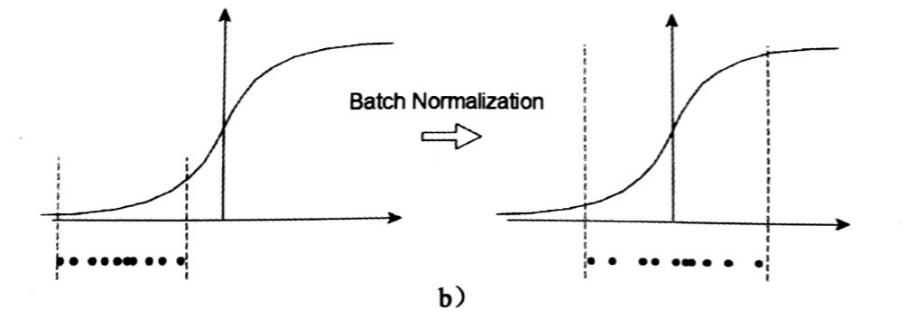
\includegraphics[width=.4\textwidth]{2.png} 
	\caption{2-dimension}  %图片的名称
	\label{fig:f2}   %标签,用作引用
\end{figure}

\subsection{Dropout}
Like its name, neurals will be dropped temporarily from network according to probability p. By this method, people solved the problem of overfitting and make our network more robust.

It works at the training stage.

\begin{figure}[h]
	\centering  %插入的图片居中表示
	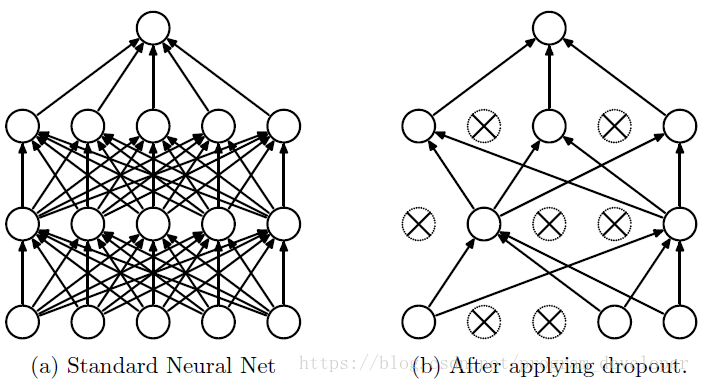
\includegraphics[width=.4\textwidth]{1.png} 
	\caption{2-dimension}  %图片的名称
	\label{fig:f1}   %标签,用作引用
\end{figure}

Without dropout:
\begin{center}
${\displaystyle z_i^{l+1}=W_i^{l+1}y_i^l+b_i^{i+1}}$

${\displaystyle	y_i^{l+1}=f(z_i^{l+1})}$
\end{center}
With dropout:
\begin{center}
${\displaystyle r_i^j \sim Bernoulli(p)}$

${\displaystyle \tilde{y}_i^{l} = r^l*y_i^l}$

${\displaystyle z_i^{l+1}=W_i^{l+1}\tilde{y}_i^l+b_i^{i+1}}$

${\displaystyle y_i^{l+1}=f(z_i^{l+1})}$
\end{center}

\subsection{some results}
\begin{figure}[htbp]
	\centering  %插入的图片居中表示
	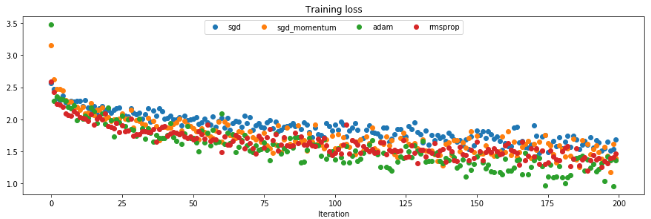
\includegraphics[width=1\textwidth]{4.png} 
	\caption{iterations}  %图片的名称
	\label{fig:f4}   %标签,用作引用
\end{figure}
\begin{figure}[htbp]
	\centering  %插入的图片居中表示
	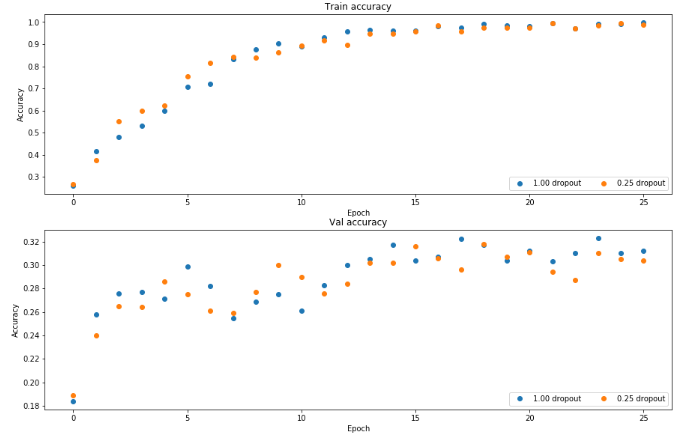
\includegraphics[width=1\textwidth]{5.png} 
	\caption{iterations}  %图片的名称
	\label{fig:f5}   %标签,用作引用
\end{figure}

\begin{figure}[htbp]
\centering  %插入的图片居中表示
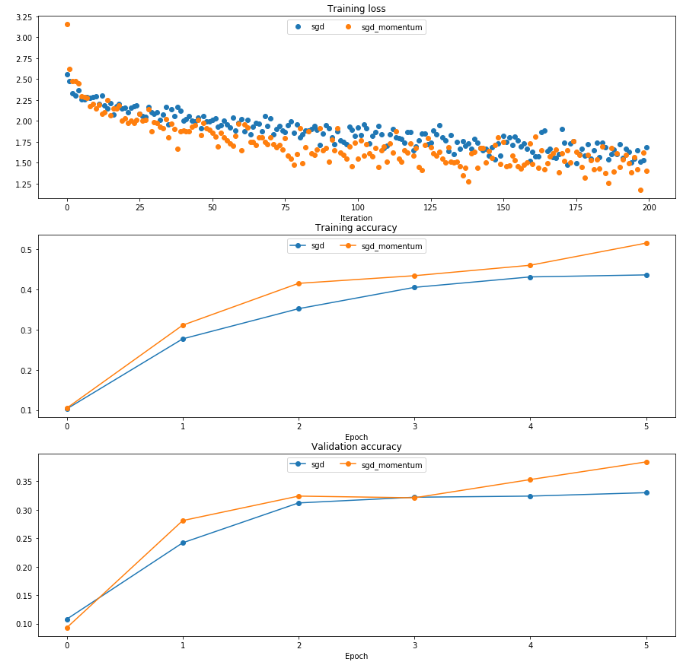
\includegraphics[width=.7\textwidth]{3.png} 
\caption{iterations}  %图片的名称
\label{fig:f32}   %标签,用作引用
\end{figure}
\section{Plan}
Next week, I will learn CNN and keep finishing assignment2. Thanks for your reading.
\end{document}